\chapter{Introduction}

% Why was the study undertaken i.e. why was this paper written?
% Proper acknowledgements of previous works
% Focus on thesis question(s)
% All cited sources should be directly relevant to the goals of the thesis
% Explain the scope. What will and what will not be included.
% Verbal road map of what's ahead
% Where do old work end and where do our work begin?

% The problem PCG solves.
In conjunction with increasing performance, memory and storage available on modern computers, the capacity for large amounts of varied content in games, movies, and other digital media grows respectively.
However, the capability to manually produce interesting content that can fully utilize this potential remains a slow and expensive process.
Consequently, many companies have decided to leverage the use of algorithms to partly, and sometimes completely, automate the production of such digital content.
These algorithms are part of a broad research field within computer science called Procedural Content Generation (PCG) \cite{pcg_in_games}.

This thesis explores the usage of PCG algorithms in order to find a suitable approach for procedural generation of modern 3D cities.
The investigation is conducted through the development of a user-friendly desktop application that can interactively generate and export models of 3D cities.
These models can then be used in third-party modeling software and game engines.
Thus, with this report we contribute with insight into various techniques applicable to city generation, as well as an open-source, MIT licensed application called \textit{CityCraft} that demonstrates such generation.

This chapter introduces the project, its goals, and some related works that have been previously done in the field of city generation.
Thereafter, follows a background chapter about the applications of PCG, and a theory chapter covering many of the fundamental techniques considered.
Finally, the project's methods and results are presented, followed up by a discussion chapter and some notes for future work.

\newpage

% Why?
\section{Purpose}

% Open-source MIT
% user-friendly standalone application
% fast and easy (generate a custom city in less than 1 minute on modern laptop)
% must work with third-party software such as Blender and Unity

Cities are complex and massive architectural infrastructures that appear all over the world, and a significant portion of the world population lives inside them.
They are also frequent scenery in digital media, such as advertisements, video games, and film.
Unfortunately, the creation of digital cities can be a highly time-consuming effort if done by hand.
Ideally, this task could be automated such that studios of any size could produce impressive cities by only specifying some rough design parameters.
The purpose of this project is to contribute towards such an ideal.

Formally, the purpose of this project is to research and combine various PCG techniques in order to discover and demonstrate a suitable approach for generating modern 3D cities. 
The intention is to demonstrate this approach by implementing a standalone city generation software, whose generated cities could be refined by artists and then integrated into medias such as video games and film.
This software should be free, open-source, and accessible to anyone in the industry of digital media.

The significance of such software compares to SpeedTree \cite{speedtree}, which revolutionized the process of creating realistic forests.
Of course, such an ambition is beyond realistic for the scope of this project, and that is why constraints have to be made.
% What and what not? I.e., what exactly?
\section{Goal and Scope}
\label{section:goal_and_scope}

The goal of this project is to develop a user-friendly application that can generate modern 3D cities and export them in a standard 3D file format such as \textit{.fbx}.
\textit{User-friendly} denotes that users should not need any technical expertise or coding experience to fully utilize the application.
Furthermore, \textit{modern cities} will be defined as cities that resemble present industrialized cities such as New York, Paris, San Francisco, and Tokyo (see Figure~\ref{fig:ModernCities}).
The intention is not to perfectly replicate these cities, but rather to draw inspiration from them.

\begin{figure}[h!]
  \centering

  \begin{subfigure}[b]{0.56\textwidth}
    \frame{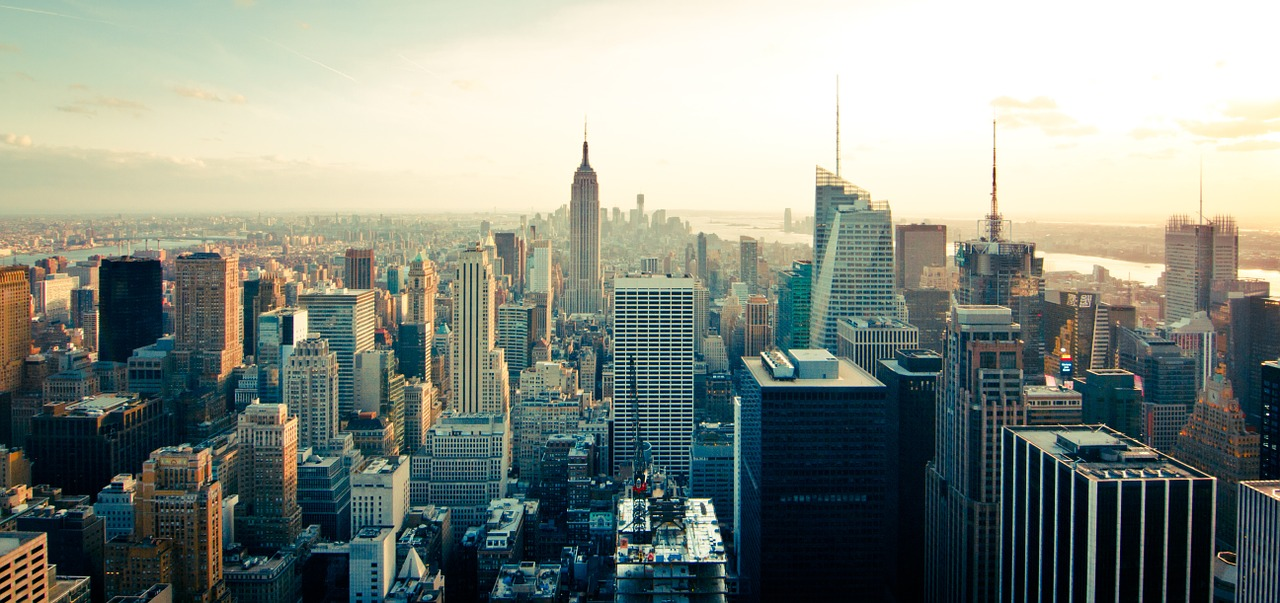
\includegraphics[width=\textwidth]{figure/modern-city-manhattan.jpg}}
    \caption{Manhattan, New York \cite{manhattan_img}.}
  \end{subfigure}
  \quad
  \begin{subfigure}[b]{0.395\textwidth}
    \frame{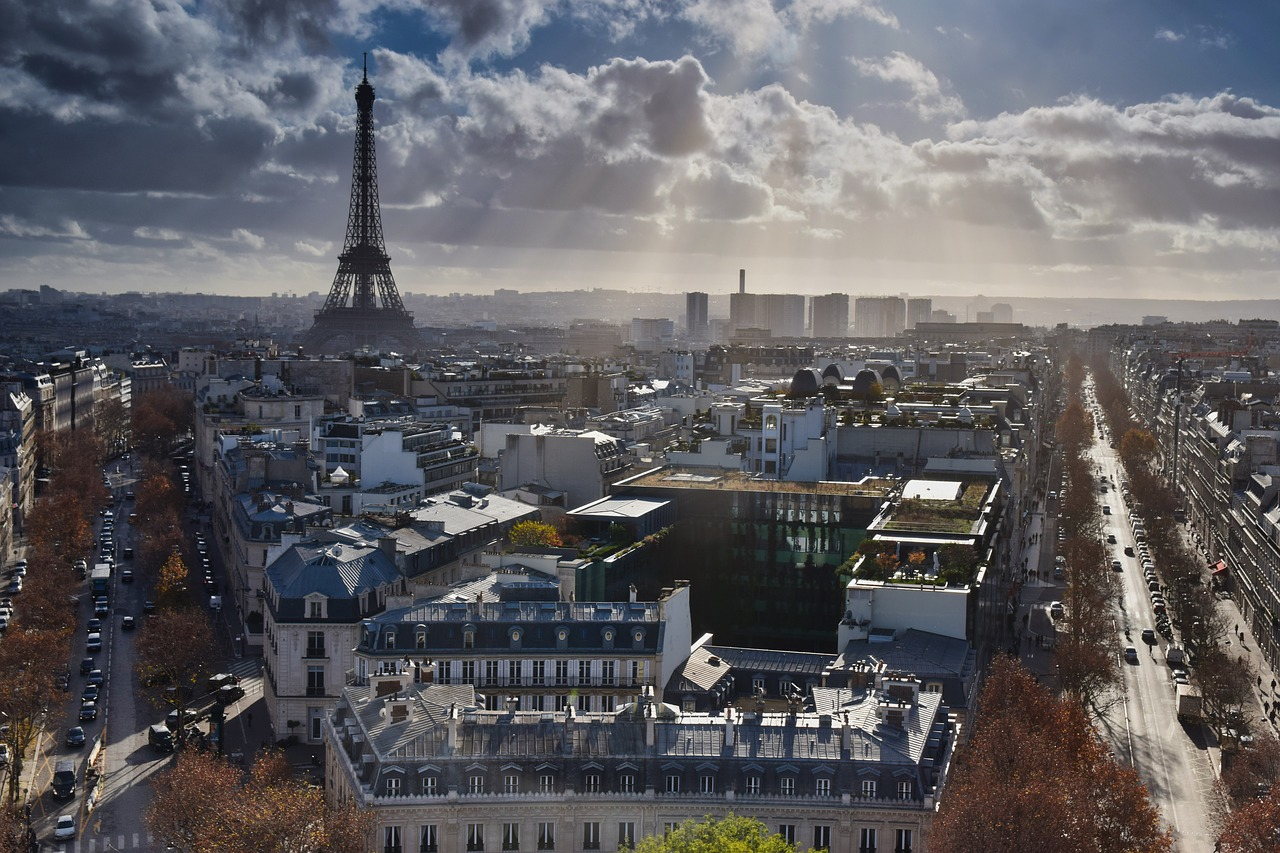
\includegraphics[width=\textwidth]{figure/modern-city-paris.jpg}}
    \caption{Paris \cite{paris_img}.}
  \end{subfigure}

  \caption{Two examples of modern cities considered in this project.}
  \label{fig:ModernCities}
\end{figure}

To clarify, suburban and rural areas are also included as part of such modern cities.

The process of generating cities should be effortless both in the sense that minimal configuration should be required, and that generation of multiple cities should be feasible within a minute from application start when running on a modern laptop.
With that said, the visual quality of models is not of immediate concern for this work.
The intention is to demonstrate a proof of concept of how PCG algorithms can be used to leverage the effort required to build cities, not to produce production-ready software.
Consequently, the use of free textures and models is encouraged in order to prioritize the development of algorithms.
Additionally, any specific art style such as low poly \cite{lowpoly_wiki} and voxel graphics \cite{voxels_wiki} is not pursued.

The generation of roads and buildings will be of primary focus, as these are considered the core features of a city.
Surrounding terrain also needs to be generated, mainly to form natural settings which the city infrastructures needs to adjust after.
Accordingly, the terrain itself does not need any significant level of detail.
Other metropolis aspects such as sidewalks, parks and parking lots are also intended to be generated, albeit with less variation.

In this contribution, generated cities will be restricted to static models in order to support integration with a wider array of third-party software.
Therefore, dynamic content such as simulation of road traffic, day-night cycles, and pedestrians are all considered out of scope.
The interior of buildings is also considered out of scope since end-users are expected to desire more control over such content than what this project's time frame can support.

As a consequence of the random and visual aspects of PCG, it is difficult to express a precise definition that can measure whether this project's final results should be considered successful or not.
Nevertheless, the following list has been constructed as a modest checklist to capture and discuss the quality of the resulting application.

\begin{easylist}
  @ \textbf{Q1} Do models correctly integrate with third-party software such as Blender \cite{blender}?
  @ \textbf{Q2} How well is the codebase structured for replacement and expansion of features?
  @ \textbf{Q3} How much notable variety is there in the generated content?
  @ \textbf{Q4} How much control do the users have over the generation?
  @ \textbf{Q5} Are the cities suitable for use in digital media such as games and film?
  @ \textbf{Q6} Are users without technical expertise able to correctly use the application?
  @ \textbf{Q7} Are there any known visual artifacts in the models?
  @ \textbf{Q8} Are there any known bugs or crashes in the application?
\end{easylist}
% Is this reasonable?
\section{Social and Ethical Aspects}

When conducting research it is vital to recognize the social and ethical implications that it might have.
This subchapter covers the major such aspects that were considered throughout this research.

The first aspect considers automation, which is a type of double-edged sword.
On one hand, the development of a city generator could lead to decreased production time and cost for game and film studios alike.
It might particularly help small production studios since they would be able to meet user expectations with less effort, and therefore better compete with the productions of larger studios.
However, this level of automation also has the potential to cause unemployment, especially in major productions where the design of large scenery might involve hundreds of employees.

Unemployment due to automation is a report on its own, but in the case of PCG, it might lead to a shift from designers towards programmers rather than job loss.
With that said, these two professions typically do not overlap in skillset.
According to game developer Scott Beca, attempting to replace level designers with PCG algorithms is ``a dangerous road to go down'' \cite{gamasutra}.
He reckons that, although significant workload traditionally done by designers might transfer to programmers, designers will still be in demand to polish and configure the building blocks used by the PCG algorithms.
Our belief is that such polish applies to the whole generation process, and therefore hope to empower designers by making the application user-friendly.

The second major aspect considers the representation of real-world cities.
If the generated cities fail to capture the various facets that compose real cities, then the generated models might pose a misleading, falsified or biased distortion of reality.
For instance, transportation facilities, history, culture, religion, poverty, politics, authorities and social injustice are all dimensions that can shape the appearance of a city.
As an example, if the generated cities do not include public transportation, does that imply that the application encourages transportation by other means?

Ultimately, a scope will have to be made, and justifying the breadth or depth of real cities within this scope will not be feasible.
Our intention is thus to only include a humble subset of the real-world dimensions, and instead encourage the contribution of further improvements by releasing the application as open-source.

To summarize, we conclude that there exist certain ethical aspects involved with the contribution of this report.
However, measures have been taken to reduce the significance of these potential risks, and with that, the proceedings involved in this research have been considered ethical.

\newpage
% What have others done?
\section{Related Works}

Generation of cities has been an active area of research for almost 20 years by now, with the \textit{Procedural Modeling of Cities} paper by Müller et al. being the pioneer \cite{muller_city_gen}.
This paper outlines the \textit{CityEngine} system, which makes heavy use of L-systems (see Chapter \ref{chap:lsystem}) to generate Manhattan-style cities from various image maps as input.
The system produces impressive results, and the paper itself proposes many interesting ideas that extend beyond L-systems.
\textit{CityEngine} later evolved into a commercial application \cite{esri}, demonstrating the real-life potential of this type of software.
Unfortunately, \textit{CityEngine} is quite expensive and remains closed-source.
Nonetheless, the original paper has been a major inspiration for our work.

Kelly and McCabe have also made significant contributions to this field with the development of \textit{Citygen} \cite{citygen_paper}, and the conduction of a prestudy \cite{citygen_paper_prestudy} summarizing common city generation techniques. 
\textit{Citygen} is an interactive system where users model cities in real-time, being heavily assisted and accelerated with the use of PCG techniques.
The paper emphasizes road generation and lot subdivision, detailing several intriguing concepts such as road graph hierarchy, snap algorithms for road segments, and strategies for building roads between significant elevation differences.

A tendency found amongst early work on road generation is that L-systems have frequently been used.
Another common approach has been agent-based generation \cite{agent_based_roads}, especially in more recent work \cite{tmwhere} \cite{robin}.
Recently, there have also been some experimentation done using the WaveFunctionCollapse (WFC) algorithm \cite{wavefunc} to generate roads \cite{wavefunc_roads}.
However, it remains difficult to determine WFC's potential compared to previous approaches as more research needs to be done \cite[p.50]{wavefunc_roads}.

Outside of academia, there has also been promising work done related to city generation.
A decade-old tech demo from \textit{Introversion Software} shows a promising generation of the outline of a city, complete with a graphical interface \cite{subversion}.
The \textit{SceneCity} plugin for Blender \cite{blender} is able to produce highly detailed buildings connected by grid-based roads \cite{scenecity}.
Impressive PCG cities can also be found in modern games such as \textit{Marvel's Spider-Man} \cite{pcg_spiderman} and \textit{The Sinking City} \cite{pcg_sunken_city}.

Unfortunately, most progress towards city generation so far remains closed-source and behind paywalls.
Exceptions exist but tend to be deprecated or incomplete solutions.
Our contribution aims to deviate from this by being open-source, free, and able to generate cities complete with terrain, roads, and buildings.
With this, we believe that the progress of city generation will be more accessible to industry and academia alike.
Accordingly, ideas presented in previous work will be combined in various ways to produce a complete, standalone city generation software.